\section{Foreground Calibration Method}
\label{sec:foreground-calibration}

This section details the foreground calibration introduced in Section II: the workflow, the control law, and the parameter set used for every reported measurement.

\subsection{Calibration Workflow}

% Editable paper diagram source: imagenes/psoc_foreground_calibration_flow_compressed.drawio (page 2)
\begin{figure}[!t]
    \centering
    
\includegraphics[width=0.90\columnwidth]{imagenes/psoc_foreground_calibration_flow.drawio.png}
    \caption{Foreground calibration flow: stored-code verification, sequential trimming, and acquisition.}
    \label{fig:calibration_flow}
\end{figure}

The calibration workflow is illustrated in Fig.~\ref{fig:calibration_flow}. At boot, after a gain change, or on command, the firmware loads the stored DAC codes and verifies whether the previously established calibration remains valid. Since DC estimation assumes a stationary geophone and slowly varying internal states, a valid operating point immediately returns the system to acquisition. Otherwise, the PGA, BP, SUM, and LP stages are calibrated sequentially with filter reset and settling after each stage. A watchdog timer and sample-count limits bound the process; during acquisition, the controller remains inactive, the LP stage is selected, and the VDAC codes remain constant.

During calibration, the programmable digital filter operates as a 128-tap FIR DC estimator, whereas during acquisition it is reconfigured with coefficients matched to the geophone bandwidth. After calibration, the acquisition coefficients, filter state, and routing are restored. A gain-indexed EEPROM record stores the valid-stage mask, four DAC codes, version, and cyclic-redundancy check (CRC); failed calibrations retain their bounded best codes without overwriting a valid record. Fig.~\ref{fig:digital_hardware} shows the digital hardware implementing this workflow.

\begin{figure*}[t]
	\centering
	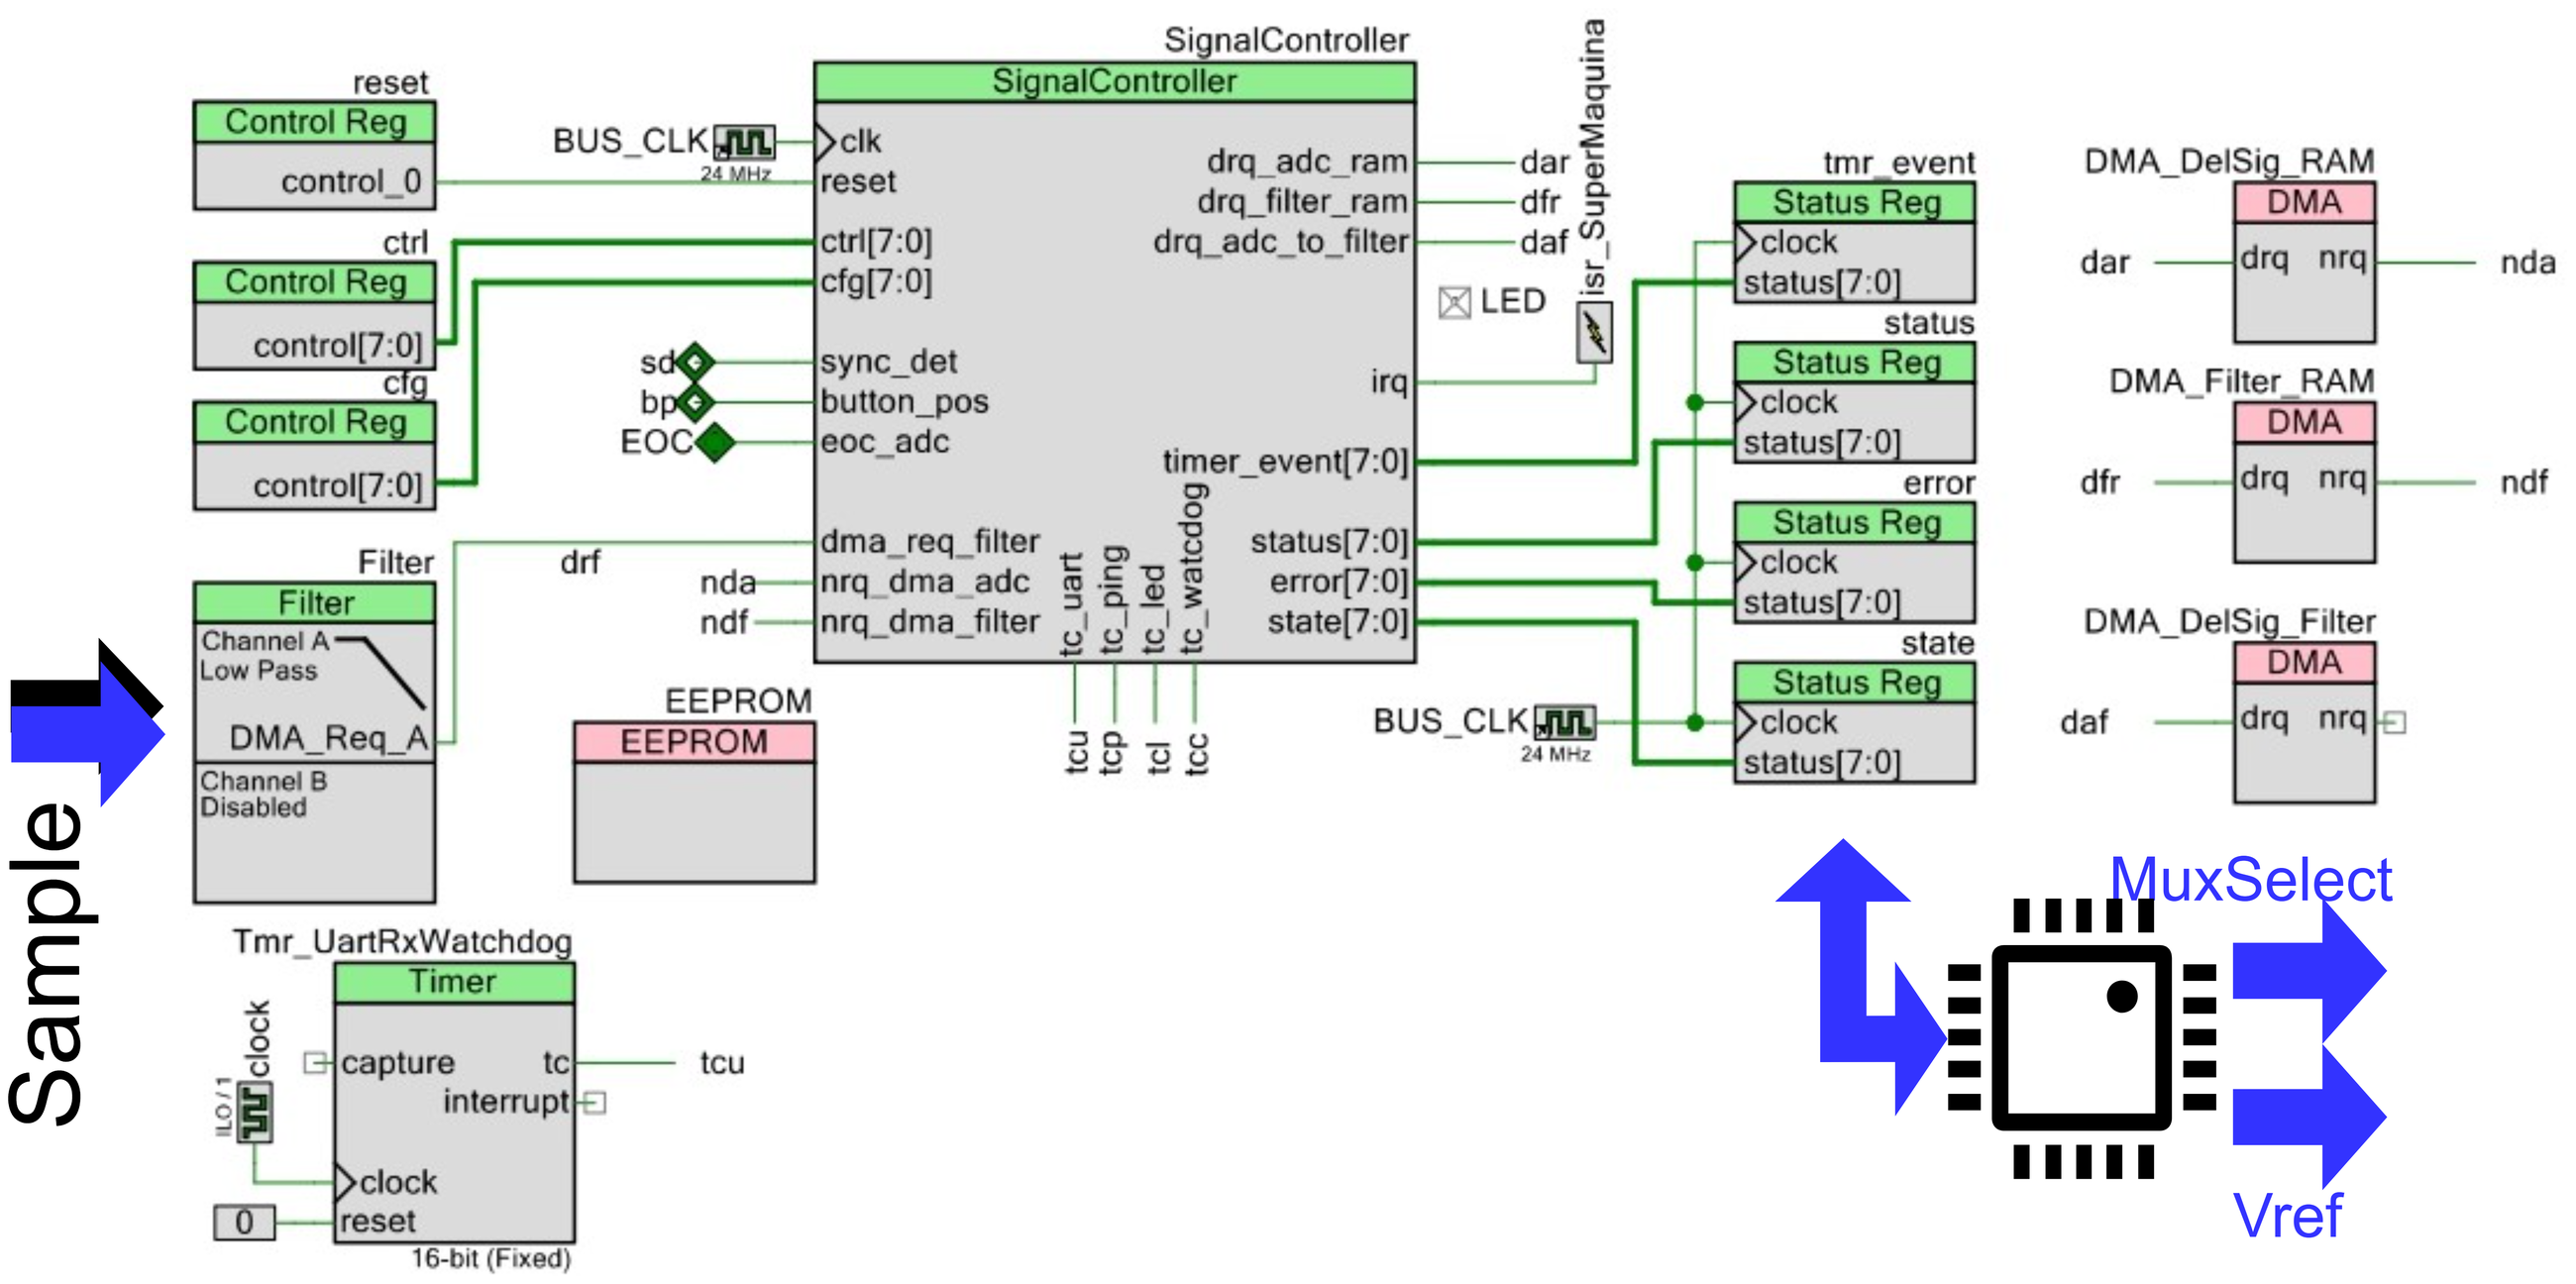
\includegraphics[width=0.90\textwidth]{imagenes/DigitalPathFinal_trim.png}
	\caption{Core PSoC digital hardware implementing the calibration workflow: signal controller, programmable digital filter, DMA channels, status registers, and EEPROM record.}
	\label{fig:digital_hardware}
\end{figure*}

\subsection{Control Law and Calibration Parameters}

The same control framework is independently applied to each analog stage. For stage $i$, $\hat{y}_i[n]$ is the filtered signed ADC count, $r_i$ is the desired reference count, and $e_i[n]$ is the residual. Since the calibration target is the reference level, $r_i=0$ and therefore $e_i[n]=\hat{y}_i[n]$. The residual is first mapped to the 8-bit DAC domain:

\begin{equation}
 \begin{aligned}
 \varepsilon_i[n]
 &= \operatorname{round}\!\left(e_i[n]\frac{q_{\mathrm{ADC}}}{q_{\mathrm{DAC}}}\right)\\
 &= \operatorname{round}\!\left(
 \frac{e_i[n]V_{\mathrm{ADC,span}}N_{\mathrm{DAC}}}
 {N_{\mathrm{ADC}}V_{\mathrm{DAC,span}}}\right),
 \end{aligned}
 \label{eq:scale}
\end{equation}

where $q_x=V_{x,\mathrm{span}}/N_x$ is the quantization step and $N_x$ the number of quantization levels. Nominal datasheet values are used throughout: $N_{\mathrm{ADC}}=2^{18}$, $N_{\mathrm{DAC}}=2^8$, $V_{\mathrm{ADC,span}}=5000$~mV, and $V_{\mathrm{DAC,span}}=4096$~mV, giving $q_{\mathrm{ADC}}=5000/2^{18}$~mV/count and $q_{\mathrm{DAC}}=16$~mV/code \cite{InfineonPSoC,InfineonAN60305}.

Equation~\ref{eq:scale} produces an integer error in equivalent DAC codes. To avoid oscillation between adjacent codes when the ideal operating point is not realizable, the implementation adopts the conservative one-step floor

\par\noindent
\begin{minipage}[c]{0.45\columnwidth}
\footnotesize
\begin{equation}
 \Delta_{i,\min}^{\mathrm{impl}}=\max(1,\lceil|K_i|\rceil),
 \label{eq:deadband}
\end{equation}
\end{minipage}%
\hfill
\begin{minipage}[c]{0.54\columnwidth}
\footnotesize
\begin{equation}
 \bar{\varepsilon}_i[n]=
 \begin{cases}
 0, & |\varepsilon_i[n]|\leq\Delta_i,\\
 \varepsilon_i[n], & \text{otherwise},
 \end{cases}
 \label{eq:deadband-error}
\end{equation}
\end{minipage}
\par

Inside the deadband, Eq.~\ref{eq:deadband-error} suppresses integration, while lock and refinement determine convergence. Table~\ref{tab:cal_params} lists the adopted values satisfying $\Delta_i\geq\Delta_{i,\min}^{\mathrm{impl}}$.

Under the assumptions of Section~\ref{sec:platform-design}, the DA-AFE requires a measurable stage output together with sufficient trim authority and range. The controller is implemented in positional proportional-integral (PI) form,

\begin{equation}
c_i^*[n]=c_{i,\mathrm{base}}-s_i\left[
 \frac{k_{\mathrm{P},i}}{|K_i|}\bar{\varepsilon}_i[n]+\frac{k_{\mathrm{I},i}}{|K_i|}
 \sum_{q=0}^{n-1}\bar{\varepsilon}_i[q]\right],
 \label{eq:pi}
\end{equation}

where $c_{i,\mathrm{base}}$ is the baseline feedforward code and $s_i=\operatorname{sgn}(K_i)$. The integral term accumulates accepted residuals and resets inside the deadband. The VDAC-to-node gains $|K_i|$ were obtained by symbolic DC analysis of each stage in MATLAB, from the nominal component values of Fig.~\ref{fig:analog_path}. For the two-op-amp instrumentation amplifier PGA \cite{CypressAN60319} the resulting ratio is unity, so $K_{\mathrm{PGA}}=1$.

The command is clipped to the configured 0--255 DAC range. At either limit, integration is suspended whenever the residual would drive the command farther into saturation, preventing windup. Convergence requires a fixed number of consecutive in-deadband samples, while an adjacent-code trial is retained only if it reduces the filtered residual. At timeout, the best code is preserved and the stage is flagged.

\begin{table}[t]
\caption{Parameters used for the reported measurements. Deadbands are in equivalent DAC codes; S/L/R are settle/lock/refine samples at 2604~Hz, whereas Timeout is in seconds.}
	\label{tab:cal_params}
	\centering
	\scriptsize
	\setlength{\tabcolsep}{2.0pt}
	\resizebox{1.00\columnwidth}{!}{%
		\begin{tabular}{lccccccc}
			\toprule
			Stage & $|K_i|$ & $\Delta_{i,\min}^{\mathrm{impl}}$ & $\Delta_i$ & $k_{\mathrm{P},i}$ & $k_{\mathrm{I},i}$ & S/L/R & Timeout (s)\\
			\midrule
			PGA & 1 & 1 & 18 & $10^{-3}$ & $3\times10^{-4}$ & 512/512/1024 & 11.5\\
			BP  & 1 & 1 & 3 & $10^{-4}$ & $5\times10^{-4}$ & 512/1024/1024 & 17.3\\
			SUM & 7.89 & 8 & 10 & $10^{-4}$ & $5\times10^{-4}$ & 512/512/1024 & 11.5\\
			LP  & 6 & 6 & 8 & $10^{-4}$ & $5\times10^{-4}$ & 1024/1024/2048 & 17.3\\
			\bottomrule
		\end{tabular}%
	}
\end{table}


The parameter set in Table~\ref{tab:cal_params} was selected empirically during preliminary bench tests and subsequently kept fixed for all reported measurements. No systematic optimization was performed, demonstrating robust operation with a single controller configuration across all evaluated boards and gain settings. Section~\ref{sec:pga-note} discusses the selected value of $\Delta_{\mathrm{PGA}}=18$. Finer trim resolution could be achieved through current-output DACs or buffered injection topologies \cite{InfineonAN60305} without modifying the foreground calibration method.
